% Szablony LaTeX dla przestrzeni fazowej Conformal MIS

% Przykład 1: Pojedynczy przekrój tau = 0.25 fm/c (dims vs pr)
\begin{figure}[htbp]
    \centering
    \begin{subfigure}[b]{0.48\textwidth}
        \centering
        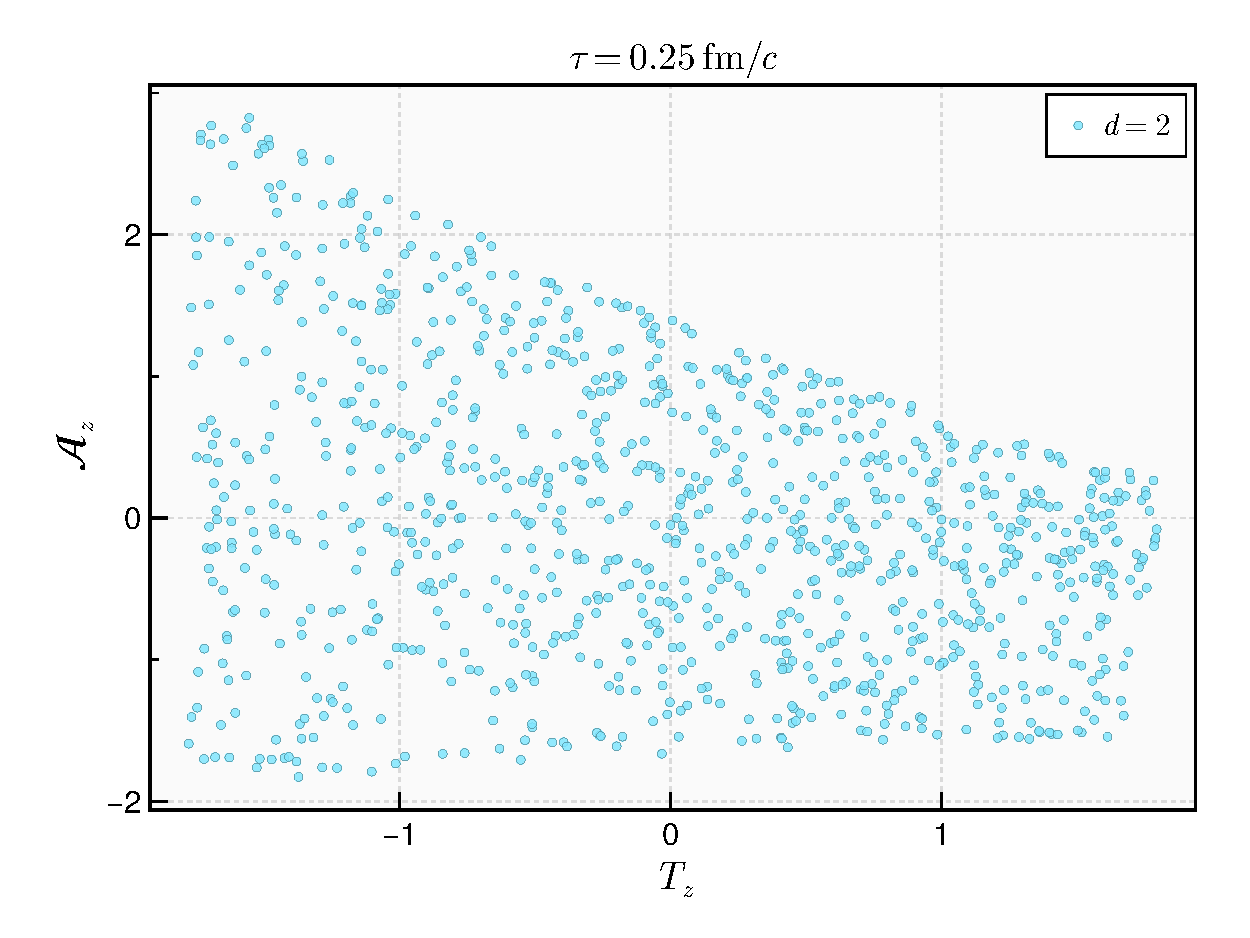
\includegraphics[width=\linewidth]{phase_space/mis/mis_zscore_slice_tau_0.25_dims.pdf}
        \caption{MIS: \emph{dims} ($\tau = 0.25\,\mathrm{fm}/c$)}
    \end{subfigure}
    \hfill
    \begin{subfigure}[b]{0.48\textwidth}
        \centering
        \includegraphics[width=\linewidth]{phase_space/mis/mis_zscore_slice_tau_0.25_pr.pdf}
        \caption{MIS: \emph{pr} ($\tau = 0.25\,\mathrm{fm}/c$)}
    \end{subfigure}
    \caption{Przestrzeń fazowa Conformal MIS w chwili $\tau = 0.25\,\mathrm{fm}/c$ w standaryzacji Z-Score.}
    \label{fig:mis_phase_space_tau_025}
\end{figure}

% Przykład 2: Zestawienie 3 wybranych chwil czasowych obok siebie
\begin{figure}[htbp]
    \centering
    \begin{subfigure}[b]{0.32\textwidth}
        \centering
        \includegraphics[width=\linewidth]{phase_space/mis/mis_zscore_slice_tau_0.20_dims.pdf}
        \caption{$\tau = 0.20\,\mathrm{fm}/c$}
    \end{subfigure}
    \hfill
    \begin{subfigure}[b]{0.32\textwidth}
        \centering
        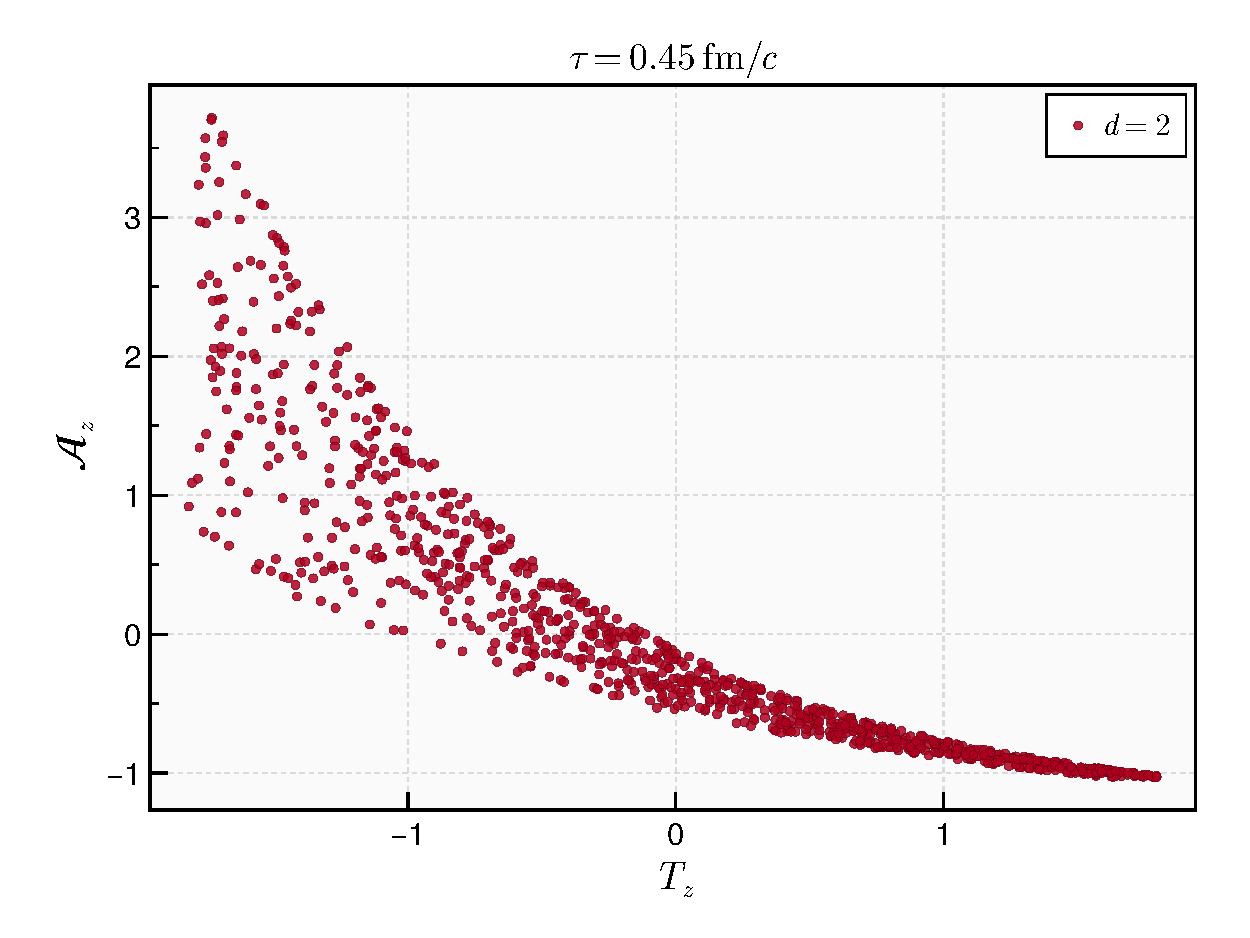
\includegraphics[width=\linewidth]{phase_space/mis/mis_zscore_slice_tau_0.45_dims.pdf}
        \caption{$\tau = 0.45\,\mathrm{fm}/c$}
    \end{subfigure}
    \hfill
    \begin{subfigure}[b]{0.32\textwidth}
        \centering
        \includegraphics[width=\linewidth]{phase_space/mis/mis_zscore_slice_tau_2.50_dims.pdf}
        \caption{$\tau = 2.50\,\mathrm{fm}/c$}
    \end{subfigure}
    \caption{Ewolucja i kolaps rozmaitości $2\mathrm{D} \to 1\mathrm{D}$ w modelu MIS dla $\tau \in \{0.20, 0.45, 2.50\}\,\mathrm{fm}/c$.}
    \label{fig:mis_3slices}
\end{figure}
